\chapter{Introduction}
\label{chp:intro}

A world without computers and computer networks can hardly be imagined in our modern day.
From basic tasks like communication and information retrieval to more complex functions such as running businesses, managing global logistics, and advancing scientific research, we rely on these computers and networks to work efficiently and stay connected.
Computers are \emph{programmable}, meaning that one can give them an arbitrary list of instructions --- a recipe if you will --- according to which they perform a large variety of functions.
When connected through networks, computers can share data, resources, and applications across the world, amplifying their power and functionality.
This combination of programmability and networking has given rise to technologies like the internet, cloud computing, and distributed systems, all of which form the foundation of today's digital world and has had a transformative impact on our society~\cite{castells_impact_2013}.
% The advancements in computing and networking technologies have given rise to a wide range of \emph{applications}, including text processing, internet browsing, emailing, video games, and mobile phone apps, but also more modern one like artificial intelligence (AI), virtual reality, and blockchain technologies.

Quantum mechanics may seem, at first glance, unrelated to computers and networks, as it primarily describes how nature behaves at the sub-atomic level.
However, quantum computers and quantum networks present opportunities for applications that are impossible on non-quantum (or \emph{classical}) computers and networks.
While classical, digital, computers and networks represent data as 0s and 1s (bits), quantum computers use quantum bits (qubits) that can exist in multiple states simultaneously, thanks to the principles of superposition and entanglement.
This allows quantum computers to perform certain calculations much faster than classical computers, such as simulation of molecular structures, fast searching, optimization algorithms, and machine learning~\cite{montanaro_quantum_2016, dalzell_quantum_2023}.
Quantum networks use quantum entanglement to realize quantum connections between its \emph{nodes}, which are quantum (computing) devices.
Using such remote entanglement as a quantum connection, quantum networks enable applications~\cite{wehner_2018_stages} including data consistency in the cloud~\cite{benor_2005_byzantine}, privacy-enhancing proofs of deletion~\cite{poremba_quantum_2022}, exponential savings in communication~\cite{guerin_exponential_2016}, or secure quantum computing in the cloud~\cite{broadbent_2009_ubqc,childs_2005_secure_qc}.
Scaling up of quantum networks is expected to result in a global \textit{quantum internet}, in which, similar to the classical internet, arbitrary quantum devices can participate and communicate with each other.


To transform a theoretical idea for a new application or use-case into an actual working implementation on computers and networks, a set of abstractions is essential.
These abstractions simplify complex software and hardware operations and allow developers to focus on designing functionality rather than dealing with low-level details.
These software abstractions include: programming languages to write the code, compilers to translate that code into machine-readable instructions, and runtime environments (such as operating systems) to execute the application.
These tools, which are widespread for classical computing and networking~\cite{aho_compilers_2006, silberschatz_book_2014, james_computer_2016}, enable the efficient use of computing and networking resources, turning high-level ideas into executable software.

For quantum computers, similar abstractions have been developed, especially in the last decade.
These include low-level instruction sets \cite{larose_overview_2019} for quantum circuits, higher-level languages for representing hybrid classical-quantum code~\cite{heim_quantum_2020}, compilers~\cite{chong_programming_2017} and full-stack runtimes for hybrid classical-quantum execution~\cite{bandic_full-stack_2022}.
Without such abstractions and tools, it would be nearly impossible to realize and scale innovative applications, whether in classical or quantum computing and networking.

% The possibility of programming arbitrary applications in high-level software has led to a lot of impact. What's more, the advent of programmable hardware and new application areas sparked novel fields of computer science research and guided further hardware development.


% qubits haven't made up their mind yet
% programs are recipes

\section{Problem statement}
For quantum networks and for a future quantum internet, however, abstractions like languages, compilers and runtimes are at present virtually non-existing.
Indeed, it is currently not possible for developers to program and execute arbitrary quantum network applications without having to deal with hardware-specific details.

Although small-scale quantum networks linking multiple quantum computing devices have recently been realized as physics experiments in laboratories~\cite{moehring_2007_ion_traps,ritter_2012_elementary,hofmann_2012_heralded,stockill_2017_phasetuned,jing2019entanglement,stephenson_2020_highrate,pompili_2021_multinode,krutyanskiy_entanglement_2023} and fiber networks~\cite{liu2024creation,stolk2024metropolitan,knaut2024entanglement}, these demonstrations so far relied either on ad-hoc software, or chose to establish that hardware parameters were in principle good enough to support a given quantum network application, although the application itself was not realized~\cite{nadlinger_device-independent_2022,liu_2022_photonic_diqkd,zhang_2022_diqkd}.
These experiments are highly technical, requiring manual manipulation of microwave pulses, lasers, and extensive knowledge of quantum physics.

In order to achieve, for quantum networks, the same level of programmability as for classical computers, classical networks and quantum computers, what is missing is hence a framework that enables
\begin{inlinelist}
\item programming quantum network application logic in a high-level, hardware-agnostic way
\item compilation of application code into low-level executable (quantum network node) machine code, and
\item execution of arbitrary applications on quantum network nodes on different kinds of hardware.
\end{inlinelist}

It is true that one can re-use existing abstractions from quantum computing, as well as from classical computing and networking, in order to realize the above framework.
However, quantum network applications present unique challenges that are not addressed by existing solutions.




\textbf{Challenge 1.} First, at the time of starting this work there simply did not exist a representation for quantum network applications, high-level nor low-level.
An initial approach at addressing this was presented with the CQC interface~\cite{dahlberg2018simulaqron}, but this is more a protocol for communication between classical and quantum devices rather than a unified programming model.
Existing quantum computing languages and compilers~\cite{heim_quantum_2020, larose_overview_2019} do not support instructions for creating entanglement with remote nodes, while these are crucial for quantum network applications.

\textbf{Challenge 2.} Furthermore, there is not yet a hardware-agnostic framework for quantum network programming.
Just as with classical and quantum computing, such an abstraction is needed to shield developers from low-level hardware details (especially since there are multiple promising technologies including color centers in diamond~\cite{ruf_quantum_2021} and trapped ions~\cite{monroe_quantum_2013, reiserer_cavity-based_2015}), enabling them to focus on application logic.

We should first highlight the difference between the quantum network applications we consider in this thesis and \emph{distributed quantum computing} (DQC)~\cite{caleffi_distributed_2024}.
The latter is a model of computation where multiple quantum computers (nodes in a network) work together to perform a quantum computation.
In this model, a quantum program (such as a single quantum circuit) is distributed (for example using circuit cutting~\cite{chatterjee_qurzon_2022}) over separate quantum computers, which use entanglement between each other in order to jointly realize the original computation.
Typically, there is a single entity that manages the circuit distribution as well as scheduling of entanglement between nodes.
For DQC there have in the recent years been developments in the creation of frameworks to program and compile such distributed quantum computations~\cite{chatterjee_qurzon_2022, cuomo_optimized_2023, ferrari_modular_2023}.

By contrast, the quantum network applications we consider in this work involve independent nodes, each of which determines which programs to run, how to compile them, and how to schedule tasks.
This is similar to the classical internet, where nodes run applications autonomously and decide when and how to interact with others.
Indeed, our model focuses more on applications for a future quantum internet, rather than on DQC.
With this distinction clear, we can consider other challenges in realizing the aforementioned needed framework for quantum network (or internet) applications.

\textbf{Challenge 3.} Quantum network applications consist of a hybrid of classical and quantum code segments.
While such hybrid code is also seen in quantum computing --- such as \textit{variational quantum eigensolvers (VQE)}~\cite{diadamo2021distributed, liu2022layer} or \textit{quantum approximate optimization algorithms (QAOA)}~\cite{farhi2014quantum} ---
these typically alternate between classical code and quantum circuits, never leaving quantum memory `live' while doing extensive classical computations.
By contrast, quantum network applications are more \textit{interactive}: classical and quantum code segments may run concurrently, communicating and influencing each other in real-time.
For instance, a quantum circuit may ``pause'' halfway, keeping quantum states in memory, and wait for a value from a classical segment (like a classical message from a remote node) before continuing.
Given the limited lifetime of quantum memories (quantum states decoherence --- decrease in quality over time)~\cite{shor_scheme_1995}, scheduling and synchronizing these interdependent quantum and classical segments is needed in order to achieve adequate application execution.

\textbf{Challenge 4.} Another crucial part of quantum network applications is entanglement generation between nodes.
Research is being done on how to realize a \emph{quantum network stack}~\cite{dahlberg2019linklayer,kozlowski2020networklayer, caleffi_2017_optimal}, which organizes entanglement generation in networks, including timing synchronization, routing, and serving application requests~\cite{gauthier_control_2023};
however, integration of applications with such a stack has not yet been implemented and studied.
Moreover, this integration requires handling both local application instructions and network-wide communication, which introduces a large span of time scales, a challenge for designing a software architecture for quantum network nodes.
Indeed, entanglement generation requires very precise (at least nanosecond) timing synchronization between the network nodes~\cite{dahlberg2019link}, while application logic, including classical messaging between nodes, may be on the order of milliseconds.

\textbf{Challenge 5.} Finally, quantum network applications often have moments in which they are idle since they have to wait for a message to arrive from another node.
Such idle times present an opportunity to do \emph{multitasking} --- running multiple applications concurrently --- on a node, in order to make more efficient use of quantum hardware.


\section{Research objective}
In this thesis, we address the gap that exists for quantum networks: namely that there is no programming and execution framework for quantum network (or internet) applications.
The main goal is to \emph{enable programming and execution of arbitrary quantum network applications in a hardware-agnostic way while optimizing runtime performance}.
We work towards this goal by addressing the following research questions:

% Main objective
% - A programmer should be able to write a quantum network application in an abstract representation (i.e. using high-level concepts without having to know details of physical realizations of quantum networks)
% - Programmers should be able to run these abstract application descriptions on real quantum networks of various hardware types, in an optimized* way, without having to do these optimizations them
% - Enable hardware-agnostic optimized execution

\begin{itemize}
  \item[Q1.] \textbf{How should quantum network applications be programmed?}
    We first address the question of how one should represent quantum network applications as programming code.
    The goal is to develop a model similar to that in classical and quantum computing, where applications have both a high-level, human-friendly representation and a lower-level, execution-oriented one.

    One challenge comes from the hybrid nature of quantum network applications, which require the integration of both classical and quantum code.
    Additionally, we aim to support a variety of hardware types.
    For the high-level representation, programmers should be able to focus on application logic without needing to understand specific hardware constraints.
    For the lower-level representation, we aim for flexibility, allowing the integration of emerging hardware platforms as they are developed.
    We do this given the uncertainty around which quantum hardware platforms will ultimately prove viable.

    Finally, the representation should be suitable for execution on quantum network nodes, leading to the next research question.

  \item[Q2.] \textbf{How should a quantum network node execute arbitrary applications?}
    Programming an application is one step; executing it on real quantum network nodes is another.

    We tackle the challenge of executing arbitrary applications --- anything a programmer might write using our representation (Q1) --- on quantum network nodes.
    Again, the hybrid nature of these applications presents a challenge: how can we effectively control the execution of both classical and quantum code?
    Additionally, we must consider how application logic (classical or quantum) should interact with the networking code.
    Another difficulty is managing and integrating the range of timescales mentioned above.
    Finally, in order to make optimal use of hardware and to increase throughput, we investigate how to enable multitasking of applications.

  \item[Q3.] \textbf{How can we improve performance of application execution?}
    A framework for programming and executing applications does not by itself guarantee optimal runtime performance.
    Application performance may be measured using classical metrics like execution time, and quantum metrics like success probability (see \cref{chp:background}).
    In general, the runtime performance of applications depends on ahead-of-time \emph{compilation} and runtime \emph{scheduling}.
    We investigate how we can perform compilation and scheduling in order to increase performance of applications.
    Especially in a multitasking scenario, scheduling has a large effect on performance.
    However, even without multitasking, the question remains of how to schedule both application code and networking tasks.

\end{itemize}


\section{Thesis outline}
With this thesis, we achieve the goal of enabling programming and execution of quantum network applications.
We do this by presenting new tools and system and software architectures.
\cref{intro:fig:chapters_overview} visualizes how these fit together.

In \cref{chp:background}, we first provide more background information about quantum internet applications.
It introduces concepts and terminology that are used in the following chapters.

In \cref{chp:netqasm}, we present NetQASM: the first programming representation for quantum network applications, addressing Q1.
This representation includes a new low-level instruction set architecture tailored to quantum network applications,
but it also contains a high-level software development kit, enabling developers to express their application logic.
We purposefully make NetQASM hardware-independent and extendible.
We also introduce a first model for execution of applications programmed using NetQASM, addressing Q2.
We evaluate our design choices in simulation.

In \cref{chp:qnodeos} we fully focus on the question of application execution (Q2).
Building on top of our execution model from \cref{chp:netqasm}, we present a detailed full-stack system architecture --- QNodeOS --- for executing arbitrary applications on quantum network nodes.
This architecture is the first of its kind.
We implement QNodeOS on a setup with two real physical quantum network nodes, and show that our architecture can successfully execute quantum network applications.
We report on the performance of our architecture by looking at application throughput and success probability.


Based on what we learned from our QNodeOS implementation and evaluation, we propose an improved architecture --- Qoala --- for executing applications on quantum network nodes in \cref{chp:qoala}.
Qoala addresses the compilation and scheduling challenges found in QNodeOS, by allowing hybrid classical-quantum compilation and scheduling.
We show how this architecture enables strategies to achieve better application performance, addressing Q3.

In \cref{chp:compiler} we discuss in more detail how Qoala can be used for improved compilation strategies.
Finally, in \cref{chp:conclusion} we conclude and reflect upon future directions.


\begin{figure}[t]
    \centering
    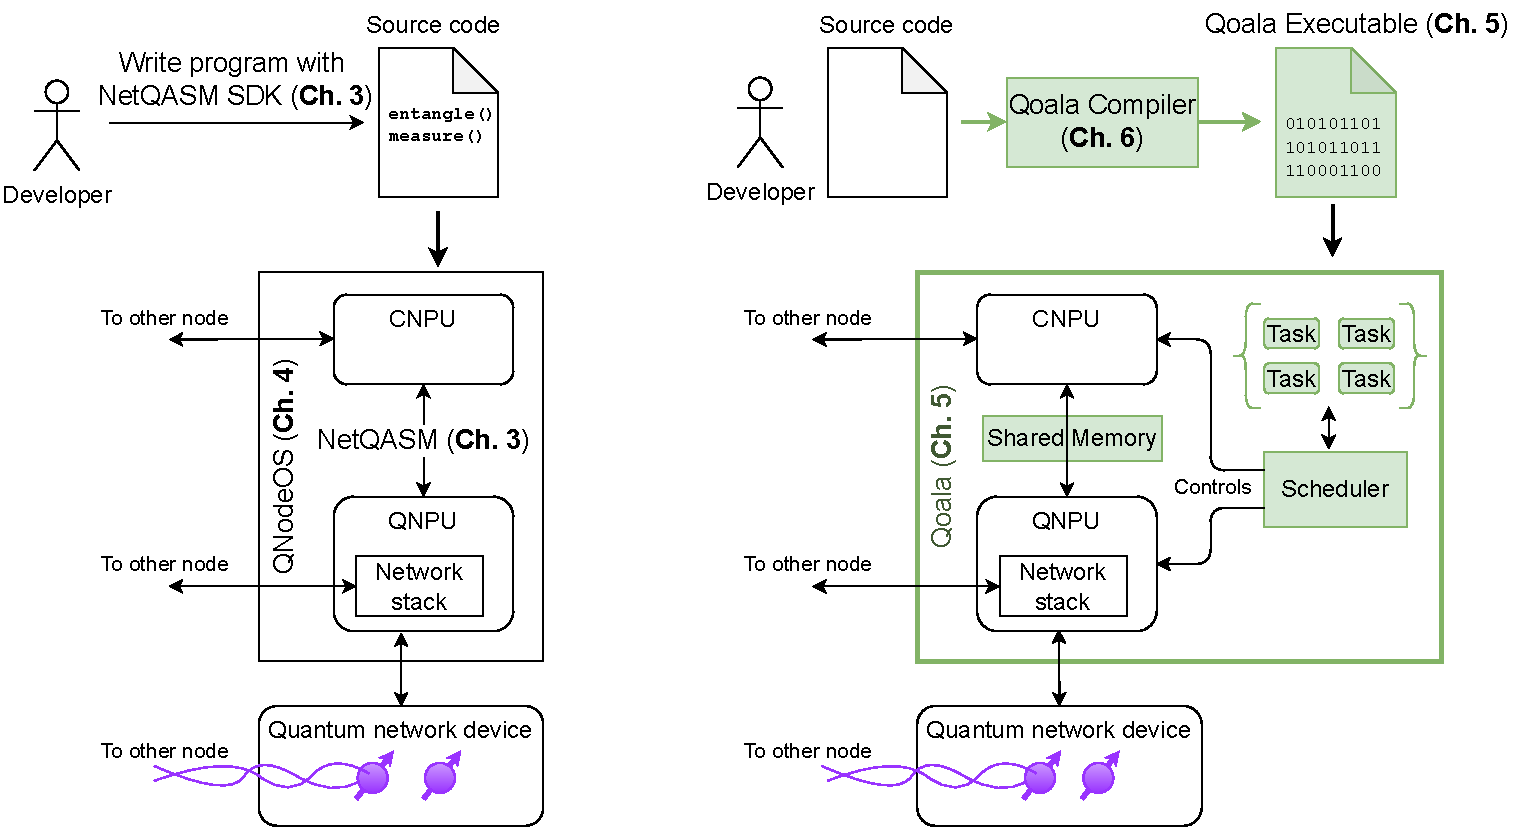
\includegraphics[width=1.0\textwidth]{figures/intro/chapters_overview.pdf}
    \caption{Visualization of how the architectures presented in this thesis fit together.
      Left: high-level schematic of a quantum network node stack. A developer writes a program using the NetQASM SDK (\cref{chp:netqasm}), which is executed by QNodeOS (\cref{chp:qnodeos}).
      QNodeOS internally uses NetQASM (\cref{chp:netqasm}) to communicate between the classical and quantum systems (CNPU, QNPU, see \cref{chp:qnodeos}).
      QNodeOS controls the quantum network device containing quantum memory (qubits, purple circles, some of which may be entangled with qubits in other nodes).
      \newline
      Right: Same quantum network node stack but with updates from \cref{chp:qoala,chp:compiler}: Qoala is an updated execution framework, still using the CNPU and QNPU, but adding a scheduler and shared memory (\cref{chp:qoala}).
      Moreover, a compiler (\cref{chp:compiler}) first converts source code into an executable, which is then executed by Qoala.
    }
    \label{intro:fig:chapters_overview}
\end{figure}




\begin{xstretch}
\printbibliography[heading=subbibintoc,title={References},notcategory=noprint]
\end{xstretch}
